\section{Pacer Data Results}

\begin{figure}[h]
\centering
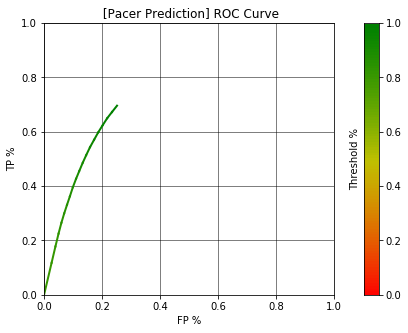
\includegraphics[width=12cm]{body/results/Graphs/PacerStuff/Raw.png}
\caption{Pacer}
\label{fig:pacer}
\end{figure}

Here we used a set of provided ``pacer data'' which contained the predictions from the predictive methods currently implemented at DraftKings. Using this dataset, we formulated the ROC in Figure \ref{fig:pacer}. As we can see, this curve is a immediately better than the baseline achieving higher True Positive rates at the same False Positive rates. For the rest of this section, we investigate what adding the pacer data to our ensemble does to the predictive performance. However, DraftKings has only just recently started collecting their pacer data so instead of 4 validation sets of data we only had 1.

\pagebreak

\begin{figure}[h]
\centering
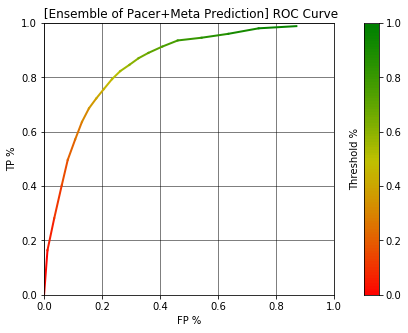
\includegraphics[width=12cm]{body/results/Graphs/PacerStuff/EnsemblePacerMeta.png}
\caption{Pacer Ensemble}
\label{fig:pacerEns}
\end{figure}

Figure \ref{fig:pacerEns} shows the ROC generated using our Header data and DraftKing's pacer data in our ensemble method. Comparatively, Figure \ref{fig:pacerFullEns} shows the ROC generated using our Header data, DraftKing's pacer data, and our KF and WLS data in our ensemble method. Both approaches seem to produce nearly equivalent curves, with the latter performing better for False Positive rates $\geq$ 0.3.

Figure \ref{fig:pacerComp} shows a comparison between both the aforementioned methods and an ensemble of just Header, WLS, and KF data relative to our baseline. Here, we can see that for nearly all False Positive rates, either the ``Pacer+Header'' or ``Header+Pacer+WLS+KF'' achieves the highest True positive rate. This would imply that the existing pacer data is helpful for improving our ensemble prediction.

\pagebreak

\begin{figure}[h]
\centering
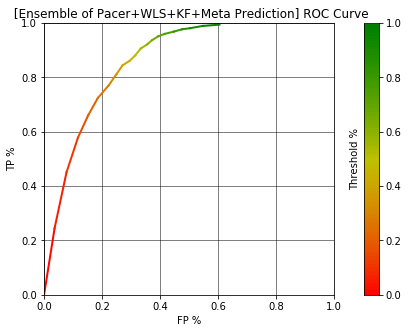
\includegraphics[width=9cm]{body/results/Graphs/PacerStuff/EnsemblePacerMetaWLSKF.png}
\caption{Pacer Full Ensemble}
\label{fig:pacerFullEns}
\end{figure}

\begin{figure}[h]
\centering
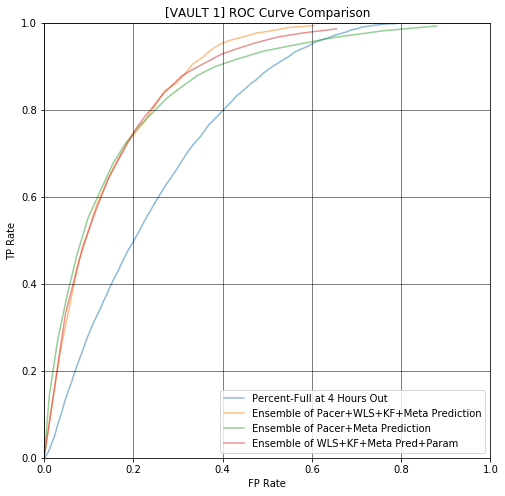
\includegraphics[width=7cm]{body/results/Graphs/PacerStuff/Compare.png}
\caption{Pacer Comparisons}
\label{fig:pacerComp}
\end{figure}

\pagebreak